% ===========================================================================
% chapters/results_and_discussions.tex — Results and Discussion
% ===========================================================================

\chapter{Results and Discussion}\label{ch:results}

This chapter is divided in two halves. The first reports the engineering output of the isothermal model: the steady-state concentration profiles of all ten species along the reactor at the design operating point, together with short parametric studies over three independent process levers --- reactor temperature, feed velocity, and side-injection mass flow. The second half benchmarks the three time-integration algorithms on the same model: wall-clock time on the real eight-reaction problem, max-norm relative error on a simplified single-reaction reactor with an analytical reference, and an explicit-vs-implicit Euler comparison at a fixed grid. The two halves are combined into a single solver recommendation at the end. The eight reactions of the kinetic model from \cref{ch:kinetic_model} are recapped in \cref{tab:reactions_recap} and referenced as R1--R8 throughout this chapter.

\begin{table}[H]
\centering
\footnotesize
\caption{The eight global reactions of the adopted kinetic scheme.}\label{tab:reactions_recap}
\begin{tabular*}{\textwidth}{@{\extracolsep{\fill}} l l l}
\toprule
 & Reaction & Process \\
\midrule
R1 & \ce{CH4 + \frac{1}{2} O2 -> CO + 2 H2}                                   & methane partial oxidation \\
R2 & \ce{C6H6 + 3 O2 -> 6 CO + 3 H2}                                          & benzene partial oxidation \\
R3 & \ce{C9H10 + \frac{9}{2} O2 -> 9 CO + 5 H2}                               & \(\alpha\)-methylstyrene partial oxidation \\
R4 & \ce{CH4 + H2O -> CO + 3 H2}                                              & methane steam reforming \\
R5 & \ce{C6H6 + 2 H2O -> 2 CO + \frac{5}{2} CH4 + \frac{3}{2} C}              & benzene steam reforming \\
R6 & \ce{C9H10 + 11.5 H2O -> 6.5 CO + 2.5 CO2 + 16.5 H2}                      & \(\alpha\)-methylstyrene steam reforming \\
R7 & \ce{C9H10 + 4 H2 -> 3 CH4 + C6H6}                                        & hydrodealkylation \\
R8 & \ce{C + H2O -> CO + H2}                                                  & soot gasification \\
\bottomrule
\end{tabular*}
\end{table}

% ===========================================================================
\section{Standardised Test Conditions}\label{sec:test_conditions}
% ===========================================================================

All runs reported in this chapter were executed on a single workstation (AMD Ryzen~7 5800X3D, 8 cores / 16 threads, \SI{32}{\gibi\byte} memory, Ubuntu~24.04~LTS) using \texttt{gfortran 13.3.0} with the flags \texttt{-O2 -Wall -Wextra -fcheck=all -std=f2018}. Standardised here does not mean that the solvers share a step size or a tolerance --- there is no single setting that means the same thing across an explicit fixed-step method, an implicit fixed-step method, and an adaptive method-of-lines solver. It means that each solver is used as it is meant to be used, and the comparison reflects what each is designed to do rather than an imposed common configuration. The per-solver defaults that anchor the three numerical tests below are listed in \cref{tab:test_conditions}; the engineering profiles are all integrated with DLSODE at its default tolerances, since the engineering content is independent of the time integrator.

\begin{table}[H]
\centering
\footnotesize
\caption{Standardised test conditions; each solver at its default configuration.}\label{tab:test_conditions}
\begin{tabular*}{\textwidth}{@{\extracolsep{\fill}}lll}
\toprule
Solver & Type & Defaults \\
\midrule
Forward Euler  & explicit fixed-step       & \(\Delta t = \SI{1}{\milli\second}\) \\
Backward Euler & implicit fixed-step       & \(\Delta t = \SI{10}{\milli\second}\); Newton tolerance \(10^{-6}\) \\
DLSODE         & adaptive method-of-lines  & \(\mathrm{mf} = 25\)\footnotemark; \(\mathrm{rtol} = 10^{-5}\), \(\mathrm{atol} = 10^{-9}\) \\
\bottomrule
\end{tabular*}
\end{table}
\footnotetext{DLSODE's method flag; \(\mathrm{mf}=25\) selects the variable-order BDF integrator with an internally-generated banded Jacobian.}

% ===========================================================================
\section{Concentration Profiles Along the Reactor}\label{sec:profiles}
% ===========================================================================

The reactor design point sits inside a multidimensional operating envelope, and three of its dimensions are tunable in principle from a control room: reactor temperature, feed velocity, and the total mass flow delivered by the side injectors. This section asks what each of those three knobs does to the steady-state product distribution. The base case fixes all three at their nominal design values and establishes the reaction-zone structure the parametric variations will then perturb; each of the following three subsections varies one knob while holding the other two fixed at the design value (\(T = \SI{1173.15}{\kelvin}\), \(u = \SI{0.516}{\metre\per\second}\), and the calibrated per-injector mass flow rates). By the end, only one of the three knobs will turn out to have a non-monotonic optimum within the tested range --- and that one is therefore the most directly useful for any future parametric optimisation of the design. All four figures share a single grid resolution (\(N_\mathrm{cells} = 200\)) and the DLSODE adaptive integrator at the defaults of \cref{tab:test_conditions}.

\subsection{Design operating point}\label{ssec:profiles_base}

\begin{figure}[H]
\centering
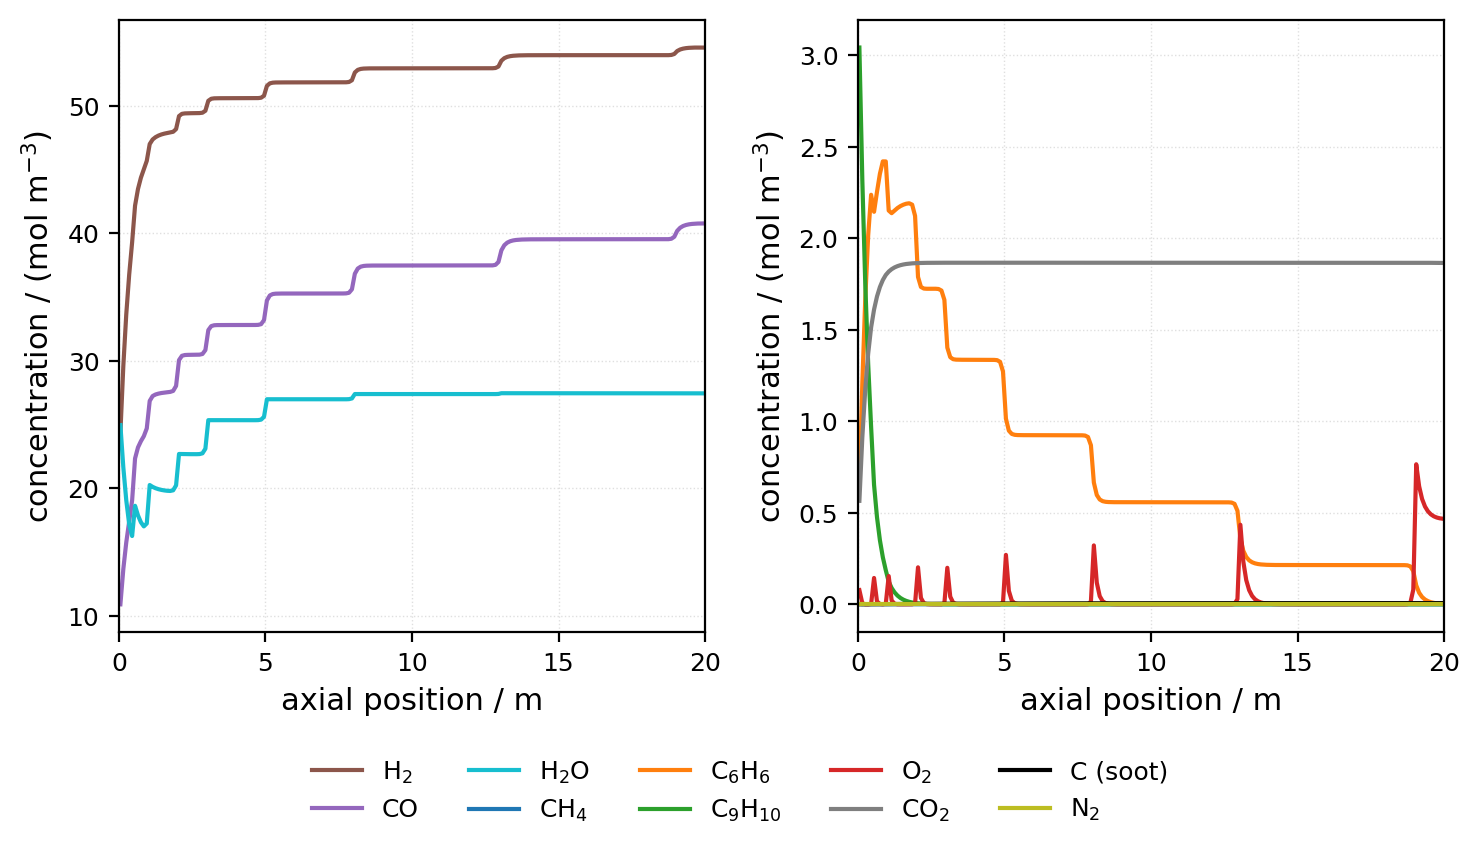
\includegraphics[width=0.95\textwidth]{figures/profiles_base.png}
\caption{Steady-state axial concentration profiles of all ten species at the design operating point (\(T = \SI{1173.15}{\kelvin}\), \(u = \SI{0.516}{\metre\per\second}\)). The two panels separate the major species (upper) from the trace species (lower) so that the two concentration scales remain legible. Methane is consumed in the first cell and does not appear in the legend.}\label{fig:profiles_base}
\end{figure}

The base case asks the simplest possible question: what does the reactor produce when all three control knobs are at their nominal design values? \Cref{fig:profiles_base} provides the answer. The two panels separate the major species (left, \SI{10}{}--\SI{55}{\mole\per\metre\cubed}) from the minor and trace species (right). Three reaction zones are visible. Within the first half-metre the pyrolytic tar precursor C\(_9\)H\(_{10}\) and the inlet methane are consumed essentially completely by partial oxidation against the dense O\(_2\) supply at the first two injectors (R1 and R3); CH\(_4\) is below its numerical floor from cell~1 onward and therefore does not appear in the legend. The two oxidation reactions emit CO, H\(_2\), and a secondary tar intermediate C\(_6\)H\(_6\), whose concentration peaks at \(\approx\SI{2.4}{\mole\per\metre\cubed}\) just downstream of the inlet bank.

Between \(x \approx \SI{0.5}{\metre}\) and \(x \approx \SI{13}{\metre}\) the reactor is in a steam-reforming regime: each O\(_2\) injector (the sharp red spikes on the right panel) is paired with an H\(_2\)O injector, and together they drive benzene oxidation, methane steam reforming, and benzene steam reforming. The combined effect is visible on every species profile as a staircase aligned with the injector positions; the C\(_6\)H\(_6\) curve in particular loses roughly half its remaining concentration at each step. From \(x \approx \SI{13}{\metre}\) to the outlet, the principal reforming and partial-oxidation reactions have run to completion: the inlet methane and \(\alpha\)-methylstyrene were consumed within the first half-metre, the benzene intermediate is below \SI{3e-3}{\mole\per\metre\cubed}, and only the last two injectors at \(x = \SI{13}{\metre}\) and \(x = \SI{19}{\metre}\) deliver small late-stage O\(_2\) and H\(_2\)O pulses to a near-depleted hydrocarbon mixture. The major-species concentrations are essentially flat, the H\(_2\)/CO ratio settles at \(\approx 1.34\), and the soot peak (right panel, C~(soot) trace) is at \(\approx \SI{0.007}{\mole\per\metre\cubed}\) --- two orders of magnitude below the active species, a clean syngas product. The N\(_2\) profile is flat by construction (inert tracer) and serves as an internal mass-balance check. With this baseline established, the next three subsections move each of the three control knobs in turn and watch what happens to the four indicator species that summarise the syngas quality: CO\(_2\), C\(_6\)H\(_6\), H\(_2\), and CO.

\subsection{Temperature variation}\label{ssec:profiles_T}

\begin{figure}[H]
\centering
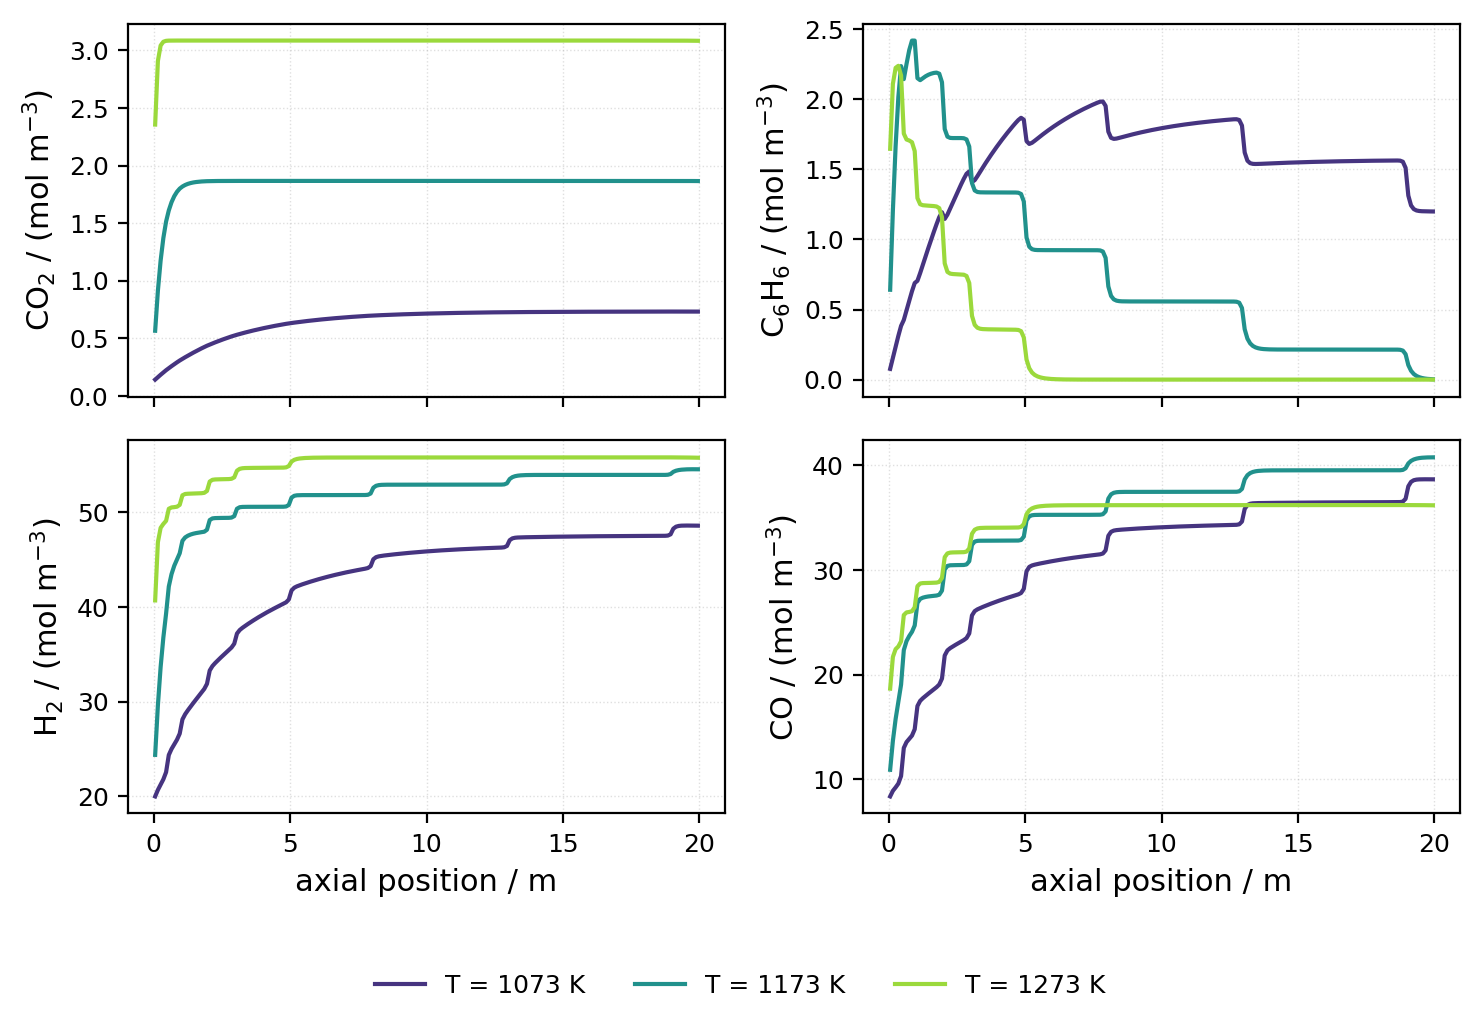
\includegraphics[width=0.95\textwidth]{figures/profiles_T_sweep.png}
\caption{Steady-state profiles of four key species (CO\(_2\), C\(_6\)H\(_6\), H\(_2\), CO) at three reactor temperatures, \(T \in \{1073, 1173, 1273\}\,\si{\kelvin}\), at the design feed velocity \(u = \SI{0.516}{\metre\per\second}\).}\label{fig:profiles_T}
\end{figure}

The first knob is the reactor temperature itself --- the most direct control in any reforming process, since every Arrhenius rate constant in the kinetic scheme depends exponentially on it. \Cref{fig:profiles_T} shows the response of the four indicator species to a \(\pm \SI{100}{\kelvin}\) excursion around the design temperature. The dominant signal is on CO\(_2\), whose outlet concentration rises monotonically from \SI{0.73}{\mole\per\metre\cubed} at \(T = \SI{1073}{\kelvin}\) through \SI{1.87}{\mole\per\metre\cubed} at the design point to \SI{3.08}{\mole\per\metre\cubed} at \(T = \SI{1273}{\kelvin}\) --- a four-fold span set by the temperature sensitivity of the \(\alpha\)-methylstyrene steam-reforming reaction (R6), which is the model's sole CO\(_2\) source. R6 has the highest activation energy of the steam-reforming family, and its rate accelerates by roughly an order of magnitude across the \SI{200}{\kelvin} range, driving the CO\(_2\) yield up in proportion. 

The temperature lever also resolves the residual-tar question: at \(T = \SI{1073}{\kelvin}\) the benzene steam-reforming reaction (R5) is too slow to consume C\(_6\)H\(_6\) within the available residence time, and a non-trivial \SI{1.2}{\mole\per\metre\cubed} of benzene arrives at the outlet --- a tar-slip regime; at \(T = \SI{1173}{\kelvin}\) consumption is essentially complete by \(x \approx \SI{15}{\metre}\); at \(T = \SI{1273}{\kelvin}\) the tar is gone within the first few metres.

The H\(_2\) outlet shows a saturating response (\(\SI{48.6}{} \to \SI{54.6}{} \to \SI{55.8}{\mole\per\metre\cubed}\)) and the CO outlet is non-monotonic (\(\SI{38.7}{} \to \SI{40.8}{} \to \SI{36.1}{\mole\per\metre\cubed}\)). The dip at the highest temperature traces back to a temperature-driven shift in the dominant \(\alpha\)-methylstyrene consumption pathway. Integrated reaction-rate diagnostics from the same runs show R3 (partial oxidation, 9 CO and no CO\(_2\) per mole of C\(_9\)H\(_{10}\)) falling from \SI{31}{\percent} of the aromatic-conversion flux at \(T = \SI{1073}{\kelvin}\) to \SI{3}{\percent} at \(T = \SI{1273}{\kelvin}\), while R6 (steam reforming, 6.5 CO and 2.5 CO\(_2\) per mole) rises from \SI{5}{\percent} to \SI{31}{\percent} over the same range. The two channels effectively swap positions; because R6 carries a CO\(_2\) coefficient that R3 lacks, the swap diverts approximately 2.5 mol of carbon per converted \(\alpha\)-methylstyrene from CO into CO\(_2\), and the CO outlet falls despite the total aromatic-conversion rate remaining unchanged. The H\(_2\)/CO ratio at the outlet shifts correspondingly from \(\approx 1.26\) at \SI{1073}{\kelvin} to \(\approx 1.54\) at \SI{1273}{\kelvin}.

In engineering terms, the design point sits just above the tar-clearance threshold: a setpoint excursion downward by \SI{100}{\kelvin} would push the reactor into a tar-slip regime, while an upward excursion of the same magnitude yields a marginally more hydrogen-rich syngas at the cost of accelerated soot formation, with the soot peak growing from \(\SI{3e-4}{\mole\per\metre\cubed}\) at \SI{1073}{\kelvin} through \(\SI{0.007}{\mole\per\metre\cubed}\) at the design point to \(\SI{0.06}{\mole\per\metre\cubed}\) at \SI{1273}{\kelvin} --- a two-orders-of-magnitude excursion across the \SI{200}{\kelvin} range.

\subsection{Feed-velocity variation}\label{ssec:profiles_u}

\begin{figure}[H]
\centering
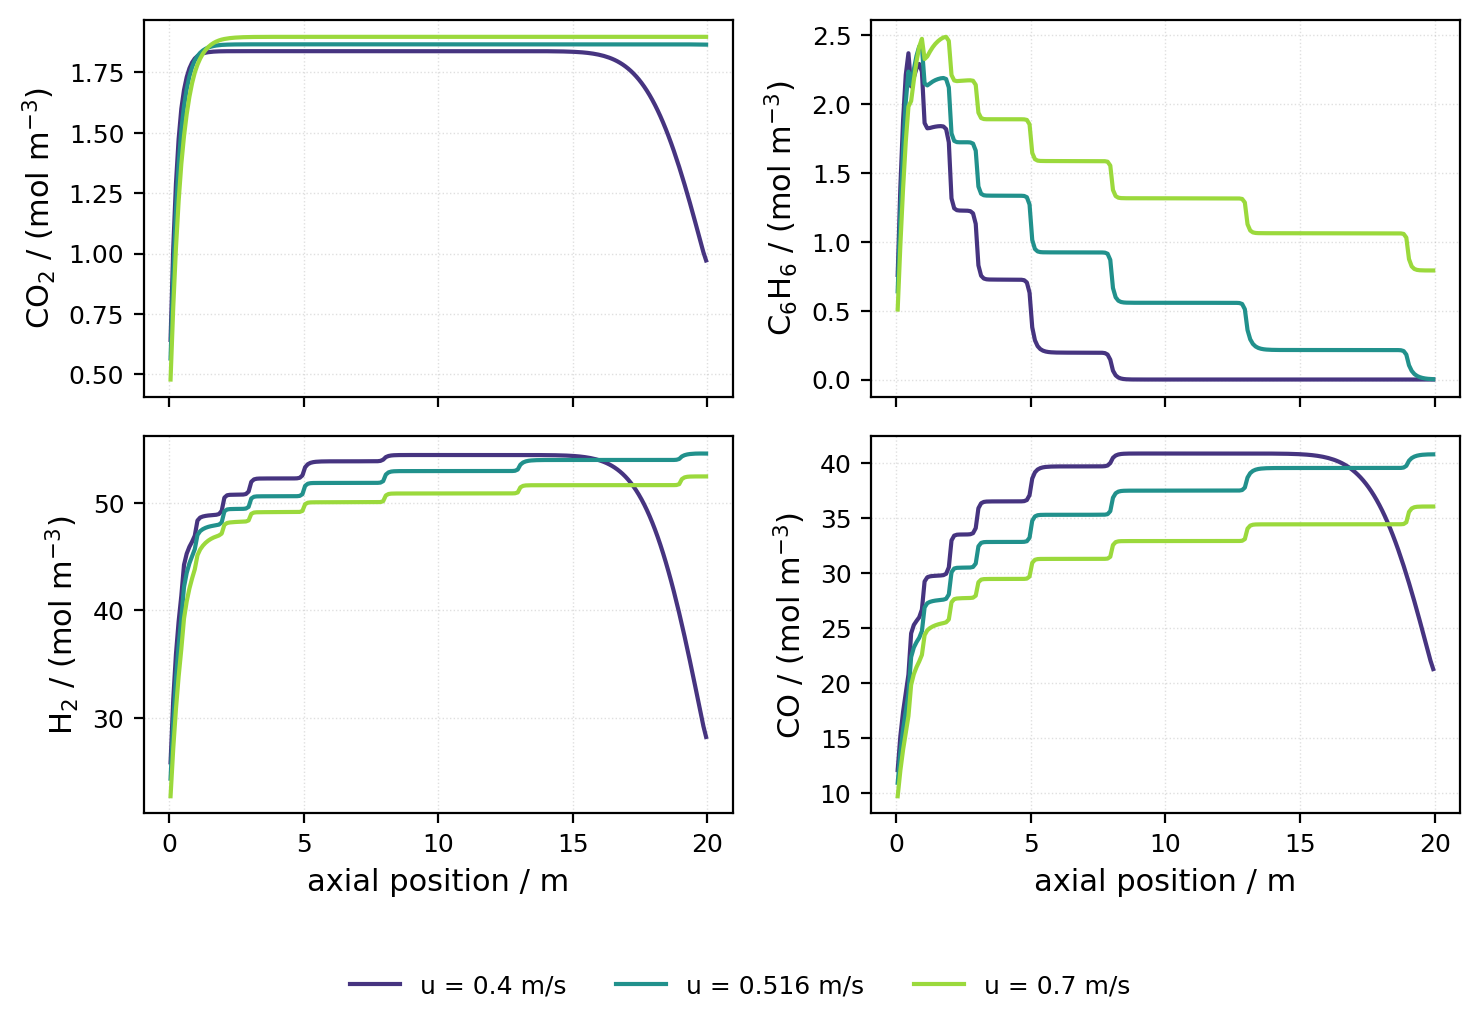
\includegraphics[width=0.95\textwidth]{figures/profiles_u_sweep.png}
\caption{Steady-state profiles of four key species (CO\(_2\), C\(_6\)H\(_6\), H\(_2\), CO) at three feed velocities, \(u \in \{0.400, 0.516, 0.700\}\,\si{\metre\per\second}\) (77~\%, 100~\%, and 136~\% of the design feed velocity, respectively), at the design temperature \(T = \SI{1173.15}{\kelvin}\).}\label{fig:profiles_u}
\end{figure}

The second knob, feed velocity, is harder to move in operation: it is set by the upstream feeder rather than the reactor itself. But moving it on paper reveals what the design value is protecting against. \Cref{fig:profiles_u} shows the response of the four indicator species to a residence-time variation of \(\tau \in \{50, 38.8, 28.6\}\,\si{\second}\), set by the inlet velocity. The clearest engineering signal is on the H\(_2\) and CO profiles at the longest residence time (\(u = \SI{0.4}{\metre\per\second}\), purple curve): both species drop sharply between \(x \approx 17\) and \SI{20}{\metre} as the last side injector at \(x = \SI{19}{\metre}\) delivers an O\(_2\) pulse that, at the slow feed velocity, finds enough downstream residence time to over-oxidise the products. 

The H\(_2\) outlet drops from a mid-reactor maximum of \(\approx \SI{55}{\mole\per\metre\cubed}\) to \SI{28.2}{\mole\per\metre\cubed} at the outlet; CO drops from \(\approx \SI{40}{}\) to \SI{21.2}{\mole\per\metre\cubed}. At the design feed velocity (teal curve) the same last-injector pulse is convected past the outlet before its O\(_2\) is exhausted, and the major-species concentrations remain essentially flat through the back half of the reactor. At the highest feed velocity (\(u = \SI{0.7}{\metre\per\second}\), green curve) the residence time is no longer sufficient to complete benzene steam reforming and \SI{0.79}{\mole\per\metre\cubed} of C\(_6\)H\(_6\) arrives at the outlet --- a partial tar-slip. 

\newpage

The feed-velocity lever therefore exhibits two competing failure modes at the extremes: over-oxidation at low feed velocity and under-conversion at high feed velocity. The design value at \(u = \SI{0.516}{\metre\per\second}\) sits in the narrow window between them where neither failure mode is active. Unlike the temperature lever, which is a candidate process knob during operation, the feed velocity is fixed by the upstream feeder and serves more as a sensitivity check on the operating design than as an active control variable. The third lever has neither limitation.

\subsection{Side-injection flow-rate variation}\label{ssec:profiles_F}

\begin{figure}[H]
\centering
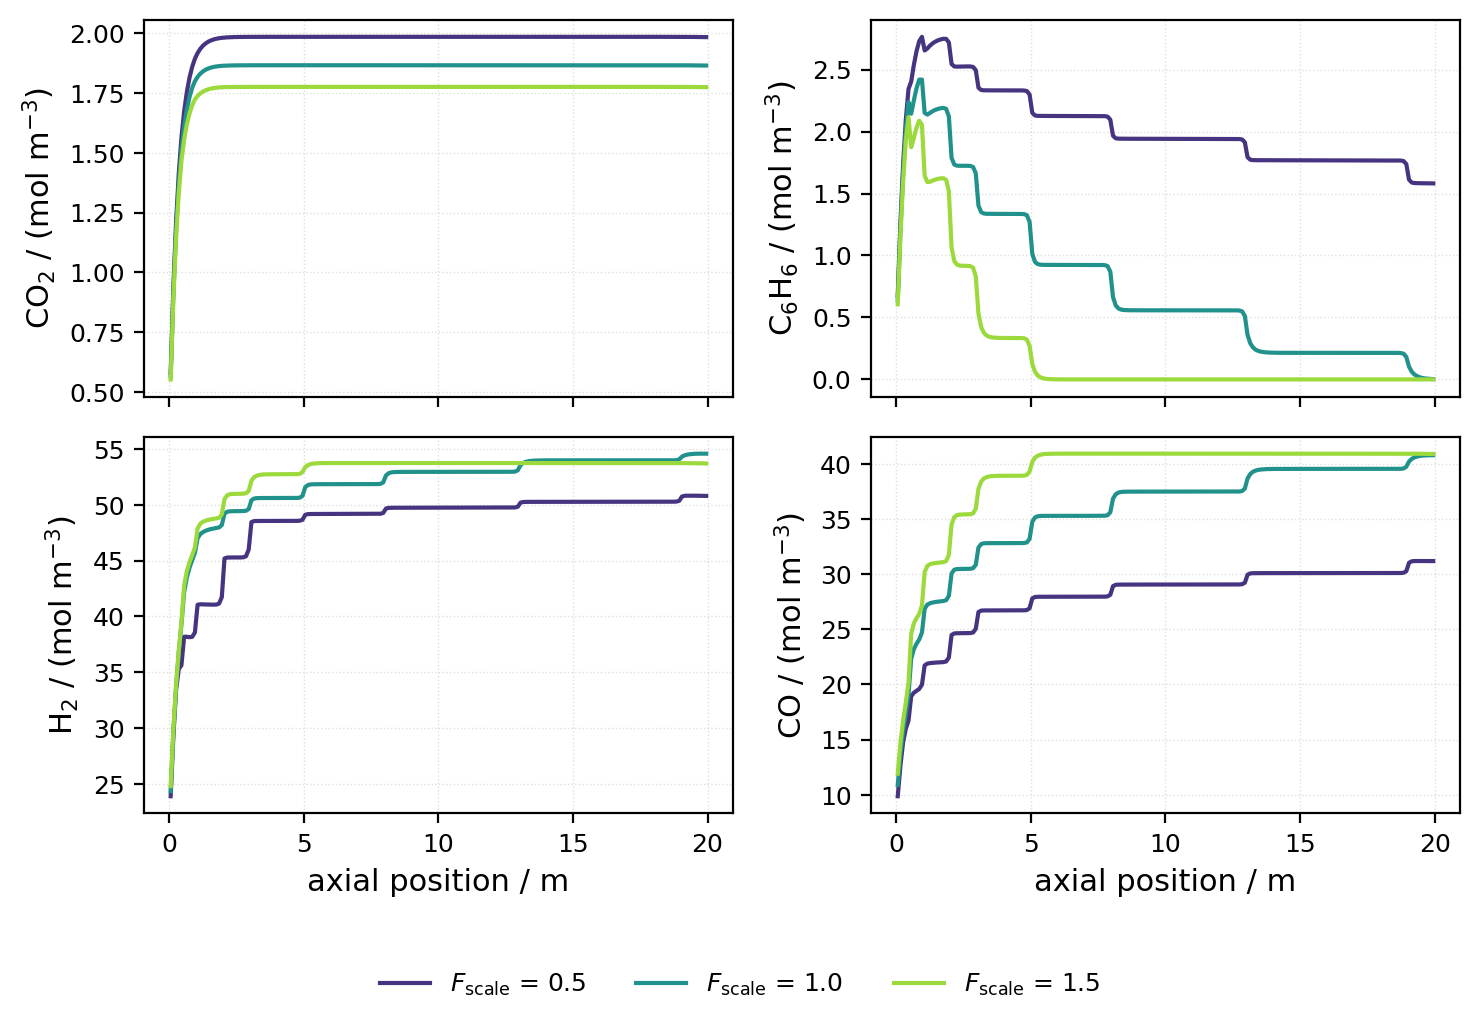
\includegraphics[width=0.95\textwidth]{figures/profiles_F_sweep.png}
\caption{Steady-state profiles of four key species (CO\(_2\), C\(_6\)H\(_6\), H\(_2\), CO) at three values of the side-injection mass-flow multiplier, \(F_\mathrm{scale} \in \{0.5, 1.0, 1.5\}\), at the design temperature and feed velocity. \(F_\mathrm{scale}\) multiplies every active injector uniformly, so the H\(_2\)O/O\(_2\) split ratio is preserved.}\label{fig:profiles_F}
\end{figure}

The third and final knob is the total mass flow delivered by the side-stream injectors. Unlike the feed velocity, it is genuinely under the reactor operator's control --- every injector has its own valve. And unlike the temperature, which lifts every Arrhenius rate uniformly, the side-injection flow probes the chemistry asymmetrically: the same multiplier hits the steam supply (which feeds reforming) and the oxygen supply (which feeds partial oxidation), so the optimum, if there is one, must come from the balance between those two channels. \Cref{fig:profiles_F} shows the response of the four indicator species to a \(\pm 50\,\%\) variation of the global side-injection mass flow. This variation differs from the \(T\) and \(u\) variations in one important respect: it exhibits a non-monotonic optimum within the tested range. 

At \(F_\mathrm{scale} = 0.5\) the under-fed reactor cannot supply enough H\(_2\)O to reform the benzene formed at the inlet, so a residual \SI{1.58}{\mole\per\metre\cubed} of C\(_6\)H\(_6\) persists along the second half of the reactor and arrives at the outlet --- a tar-slip more severe than the \(T = \SI{1073}{\kelvin}\) case; the H\(_2\) and CO outlets are correspondingly depressed (\SI{50.8}{} and \SI{31.2}{\mole\per\metre\cubed} respectively, against \SI{54.6}{} and \SI{40.8}{\mole\per\metre\cubed} at the design value). At \(F_\mathrm{scale} = 1.0\) the benzene is fully reformed by \(x \approx \SI{13}{\metre}\) and the major-species outlets reach the design-case values. At \(F_\mathrm{scale} = 1.5\) the H\(_2\) yield decreases marginally to \SI{53.7}{\mole\per\metre\cubed} while the CO outlet is essentially unchanged. 

The slight H\(_2\) drop reflects two effects of the uniform multiplier: the additional O\(_2\) delivered alongside the additional steam pushes a larger fraction of the hydrocarbon feed through the partial-oxidation channels (R1--R3), which yield fewer H\(_2\) per carbon than the corresponding steam-reforming reactions (R4--R6), and the higher overall injection flow modestly dilutes the outlet stream. Neither outlet is materially shifted, but the additional steam does suppress the soot peak from \SI{0.0066}{} to \SI{0.0026}{\mole\per\metre\cubed} (R5, the model's sole carbon-forming step, slowed relative to R8 gasification by the excess steam). 

The injection-flow rate therefore behaves as a calibration knob with a clear optimum near the design point: under-feeding starves benzene reforming, over-feeding plateaus the syngas yield while consuming additional steam-injector capacity. Of the three variations, this is the only one with a non-monotonic optimum inside the tested range. The design point sits very close to that optimum, which makes the side-injection flow rate the most directly actionable of the three control knobs for any future parametric optimisation of the reactor.

% ===========================================================================
\section{Performance: Wall-Clock vs Grid Resolution}\label{sec:walltime_test}
% ===========================================================================

The performance comparison begins with a wall-clock scaling test. The real eight-reaction isothermal reactor model is integrated from \(t = 0\) to \(t_\mathrm{end} = \SI{50}{\second}\) by each of the three solvers, at six grid resolutions, \(N_{\mathrm{cells}} \in \{50, 100, 200, 400, 800, 1000\}\). Each (solver, grid) combination is a single run; the measurement is the total CPU time reported by the integrator's internal timer, excluding output I/O.

\begin{figure}[H]
\centering
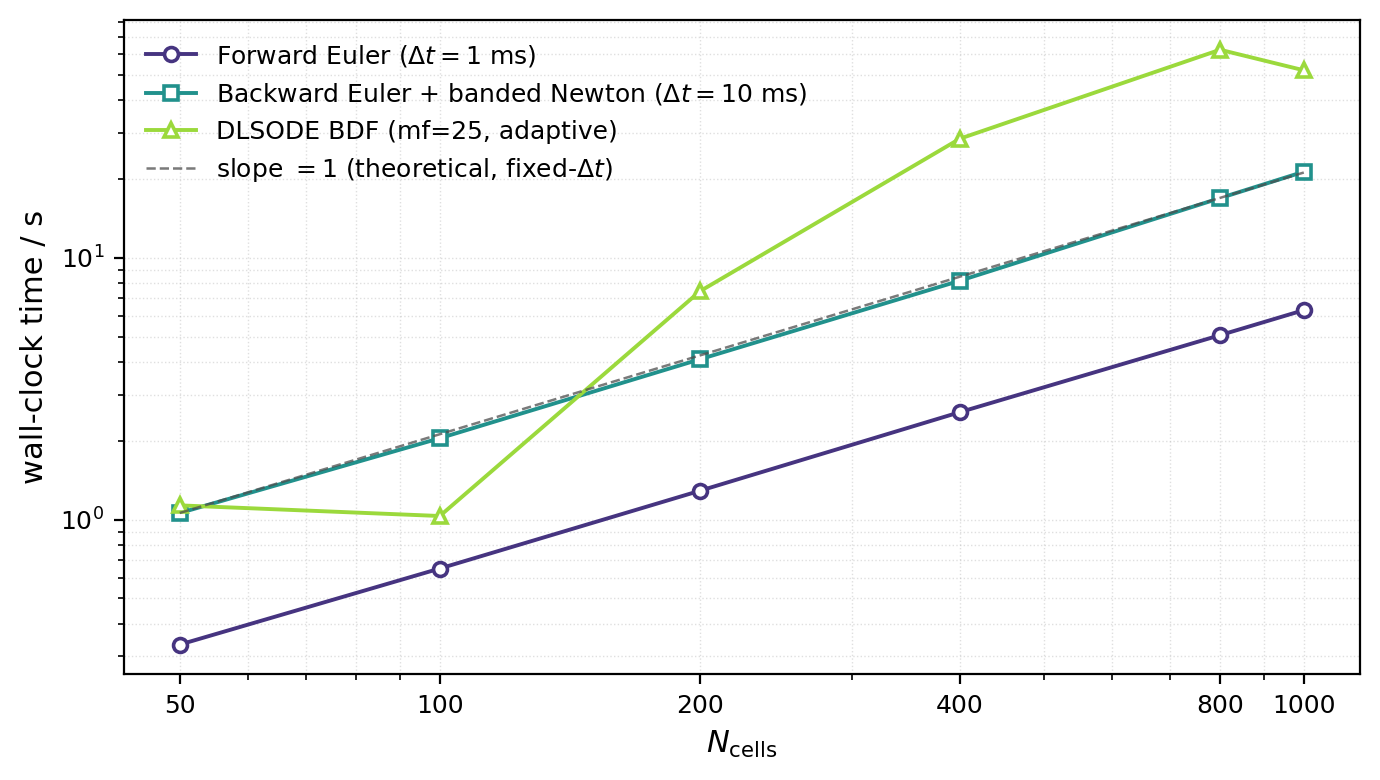
\includegraphics[width=0.95\textwidth]{figures/test1_walltime.png}
\caption{Wall-clock time vs grid resolution on the real eight-reaction isothermal reactor model, integrated to \(t_\mathrm{end} = \SI{50}{\second}\). In log-log coordinates, forward Euler and backward Euler scale linearly with \(N_\mathrm{cells}\) under fixed \(\Delta t\); DLSODE is non-monotonic, reflecting variable BDF order and adaptive step selection.}\label{fig:test1_walltime}
\end{figure}

\Cref{fig:test1_walltime} shows the result. Forward Euler and backward Euler follow the slope-one scaling expected of a fixed-\(\Delta t\) integrator on a banded right-hand side: per-step work scales linearly with \(N_\mathrm{cells}\) (banded Jacobian factorisation for backward Euler; banded RHS evaluation for forward Euler), while the step count \(t_\mathrm{end}/\Delta t\) is grid-independent. Forward Euler is roughly three times faster than backward Euler at every grid, reflecting the absence of a Newton iteration per step. 

The cube-of-\(N\) scaling that an explicit method might exhibit near the diffusive CFL boundary does not surface here: at \(\Delta t = \SI{1}{\milli\second}\) the integrator sits well below the CFL bound (\(\sim\SI{20}{\milli\second}\) at \(N_\mathrm{cells} = 1{,}000\)) throughout the sweep. DLSODE displays a non-monotonic wall-clock profile. The integrator is fastest at \(N_\mathrm{cells} = 100\) (\SI{1.03}{\second}, BDF order four), grows steadily through \(N_\mathrm{cells} = 200\) and \(400\), peaks at \(N_\mathrm{cells} = 800\) at \SI{62.4}{\second} --- slower than at the finer \(N_\mathrm{cells} = 1{,}000\) grid --- and partially recovers to \SI{52.1}{\second} at the finest resolution. 

\newpage

Inspection of the internal counters explains the peak: at \(N_\mathrm{cells} = 800\) the BDF order has collapsed to one and DLSODE has reverted in practice to backward Euler, with the internal step count rising to 22{,}856; at \(N_\mathrm{cells} = 1{,}000\) the integrator escalates BDF back to order five with substantially fewer steps. The pattern is characteristic of variable-order adaptive schemes when the local-truncation-error estimator persistently rejects high-order steps: the scheme remains A-stable but loses its order advantage, and the overhead of the predictor--corrector difference and order-selection logic sits on top of what are effectively backward-Euler numerics. DLSODE's adaptive machinery therefore provides robustness without guaranteeing monotonic performance scaling: on the present model, the integrator outperforms the fixed-step alternatives only near \(N_\mathrm{cells} = 100\) and is otherwise the slowest of the three.

% ===========================================================================
\section{Accuracy: Relative Error vs Grid Resolution}\label{sec:error_test}
% ===========================================================================

The second numerical test anchors the accuracy measurement to a closed-form analytical solution. Because the real eight-reaction model has no such reference, the test uses a simplified plug-flow reactor in which the eight Arrhenius reactions are replaced by a single first-order irreversible step, with all geometry, hydrodynamics, and discretisation choices inherited from the real model. The nine side-stream injectors are switched off for this test, so the simplified reactor receives reactant only through the Dirichlet inlet. The simplification yields a linear convection--diffusion--reaction equation whose steady-state solution is available in closed form, and the simulation--reference gap is then a clean measurement of the spatial-discretisation error of the FVM scheme that is shared by all three solvers.

\subsection{Test problem and analytical solution}\label{ssec:test_problem_analytical}

The reduced model retains the geometry of \cref{tab:reactor_params} (\(L = \SI{20}{\metre}\), \(u = \SI{0.516}{\metre\per\second}\), \(D_\mathrm{ax} = \SI{1e-2}{\metre\squared\per\second}\)), the first-order upwind FVM stencil, and the same three time-integration algorithms. Only the chemistry is replaced: the eight Arrhenius reactions of the real model reduce to a single first-order step
\begin{equation}
  \ce{A -> B}, \qquad r = k\,C_A,
  \label{eq:test2_reaction}
\end{equation}
with \(k = \SI{0.026}{\per\second}\) chosen so that the Damköhler number \(\mathrm{Da} = kL/u \approx 1\) --- the reaction timescale matches the residence time, giving a non-trivial conversion across the reactor. The Péclet number inherited from the geometry, \(\mathrm{Pe} = uL/D_\mathrm{ax} \approx 1{,}032\), places the test problem in the same strongly convection-dominated regime as the real reactor.

The steady-state mass balance for species~A is the linear ODE
\begin{equation}
  \underbrace{D_\mathrm{ax}\,\frac{\mathrm{d}^2 C_A}{\mathrm{d}x^2}}_{\text{diffusion}}
  \;-\;
  \underbrace{u\,\frac{\mathrm{d} C_A}{\mathrm{d}x}}_{\text{convection}}
  \;-\;
  \underbrace{k\,C_A}_{\text{reaction}}
  \;=\; 0,
  \qquad x \in [0, L],
  \label{eq:test2_steady_pde}
\end{equation}
subject to the same boundary conditions the FVM stencil enforces: a Dirichlet inlet \(C_A(0) = C_{A,\mathrm{in}}\) and a zero-gradient (Neumann) outlet \(\mathrm{d}C_A/\mathrm{d}x(L) = 0\). The derivation that follows is the standard reactor-engineering treatment of convection--diffusion--reaction systems, presented in detail by Levenspiel~\cite{Levenspiel1999} and Fogler~\cite{Fogler2006}. Non-dimensionalising with \(x^\ast = x/L\) and substituting the trial solution \(C_A \propto e^{\lambda\,x^\ast}\) yields the characteristic equation \(\lambda^2 - \mathrm{Pe}\,\lambda - \mathrm{Pe}\,\mathrm{Da} = 0\), whose two roots are
\begin{equation*}
  \lambda_\pm \;=\; \frac{\mathrm{Pe}}{2}\left(1 \pm \beta\right),
  \qquad
  \beta \;=\; \sqrt{1 + 4\,\mathrm{Da}/\mathrm{Pe}}.
\end{equation*}
Here \(\beta\) is the bookkeeping symbol that comes out of the quadratic equation. With our parameters (\(\mathrm{Pe} = 1{,}032\), \(\mathrm{Da} \approx 1\)) the value \(\beta = \sqrt{1 + 4/1032} \approx 1.002\) is barely above unity, and the two eigenvalues evaluate to \(\lambda_+ \approx 1{,}033\) and \(\lambda_- \approx -1\). The general solution \(C_A(x^\ast) = A\,e^{\lambda_+\,x^\ast} + B\,e^{\lambda_-\,x^\ast}\) is therefore the sum of a violently growing exponential and a gently decaying one. The growing branch reaches \(e^{1033}\) at the reactor outlet --- a number with no physical meaning in any concentration --- so its coefficient \(A\) must be of order \(e^{-1033}\), numerically zero for any practical purpose. The Neumann outlet condition pins \(A\) at exactly that level, well below the FVM discretisation errors that the test is designed to measure. Dropping the growing branch and applying the Dirichlet inlet \(C_A(0) = C_{A,\mathrm{in}}\) leaves a single decaying exponential,
\begin{equation}
  \frac{C_A(x^\ast)}{C_{A,\mathrm{in}}} \;=\; e^{\lambda_-\,x^\ast}
  \;\simeq\; \exp(-\mathrm{Da}\,x^\ast),
  \label{eq:test2_analytical}
\end{equation}
where the second equality follows from the Taylor expansion \(\beta = 1 + 2\,\mathrm{Da}/\mathrm{Pe} + \mathcal{O}(1/\mathrm{Pe}^2)\), giving \(\lambda_- = (\mathrm{Pe}/2)(1 - \beta) \simeq -\mathrm{Da}\) to leading order in \(1/\mathrm{Pe}\), and recovers the textbook plug-flow conversion law for a first-order reaction --- a useful sanity check, since at very high Péclet the dispersion term is negligible and the reactor should behave as pure plug flow. At \(\mathrm{Da} \approx 1\) this corresponds to an overall conversion of \(1 - e^{-1} \approx 63\%\). The species~B concentration follows from mass conservation, \(C_B(x^\ast) = C_{A,\mathrm{in}} - C_A(x^\ast)\). \Cref{eq:test2_analytical} is the analytical reference against which the second test measures simulation error.

The boundary conditions of the analytical reference deserve a brief note. The canonical analytical solution for steady-state convection--diffusion--reaction in a tubular reactor assumes Danckwerts (closed--closed) boundaries and is reproduced in standard reactor-engineering textbooks~\cite{Levenspiel1999}. The first-order upwind FVM does not enforce Danckwerts inlet but a simpler Dirichlet ghost cell, so a comparison against the closed--closed reference would conflate spatial-discretisation error with a constant boundary-condition mismatch of order \(1/\mathrm{Pe}\). \Cref{eq:test2_analytical} matches the boundary conditions the FVM actually applies and is therefore the cleaner reference for measuring spatial-discretisation error in isolation.

\subsection{Results}\label{ssec:test2_results}

The error metric reported below is the steady-state max-norm relative error,
\begin{equation}
  \varepsilon_\infty \;=\; \frac{\lVert C_A^{\mathrm{num}} - C_A^{\mathrm{ref}}\rVert_\infty}{\lVert C_A^{\mathrm{ref}}\rVert_\infty},
  \label{eq:max_norm_relerr}
\end{equation}
where the maximum is taken over all \(N_\mathrm{cells}\) FVM cells and the analytical reference \(C_A^{\mathrm{ref}}(x)\) of \cref{eq:test2_analytical} is independent of \(N_\mathrm{cells}\); the figure plots how the numerical solution converges to this fixed reference under grid refinement.

\begin{figure}[!ht]
\centering
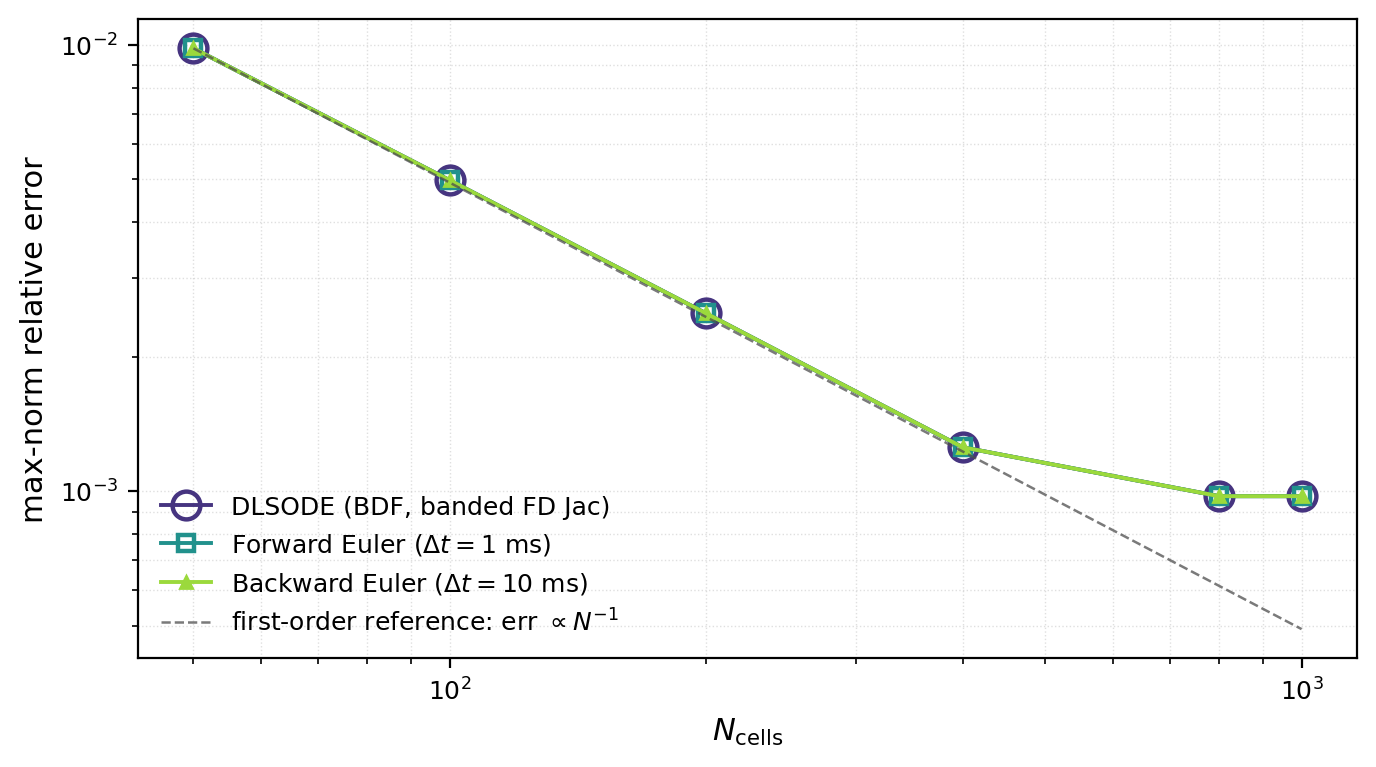
\includegraphics[width=0.95\textwidth]{figures/test2_error_vs_ncells.png}
\caption{Steady-state max-norm relative error of the simulated \(C_A\) profile against the analytical reference of \cref{eq:test2_analytical}, at six grid resolutions. The three solvers' data points overlap to four significant figures at every grid; the dashed line is the slope-(\(-1\)) reference for first-order upwind FVM.}\label{fig:test2_error}
\end{figure}

\Cref{fig:test2_error} shows the result --- and the surprise. The three solvers' data points overlap to four significant figures at every grid. Forward Euler, backward Euler, and DLSODE are accuracy-equivalent on this test at every \(N_\mathrm{cells}\) tested; the time-integration error sits below the spatial-discretisation floor for every solver, at every grid. The error trend tracks the slope-(\(-1\)) reference line closely from \(N_\mathrm{cells} = 50\) (\SI{9.82e-3}{}) to \(N_\mathrm{cells} = 400\) (\SI{1.25e-3}{}), the convergence rate predicted for the first-order upwind convection scheme. From \(N_\mathrm{cells} = 800\) onward the error plateaus at approximately \SI{9.75e-4}{}, consistent with the absolute tolerance \(\mathrm{atol} = 10^{-9}\) of the reference DLSODE run propagating into the rel-err denominator and the residual incomplete steady-state convergence at the integration window \(t_\mathrm{end} = \SI{200}{\second}\) used for this test. The overlap of the three solvers is itself the key result. On a linear test problem, the implicit Newton iteration of backward Euler converges in a single step --- the residual is exact at any \(\Delta t\) --- and the variable-order BDF formulae of DLSODE reduce in practice to backward Euler at order one; in both cases the time integration is free of truncation error to within the rounding floor, leaving only the FVM upwind scheme to set the accuracy. This is the spatial-discretisation floor: the best accuracy any of the three solvers can achieve at a given grid, regardless of how cheaply or expensively that accuracy is reached.

% ===========================================================================
\section{Explicit vs Implicit Euler Crossover}\label{sec:euler_comparison}
% ===========================================================================

The two tests above benchmark each solver at its default configuration. They do not, however, answer a more practical question: at what time step does the implicit method's per-step Newton overhead become cheaper than the explicit method's tighter step bound? This section probes that crossover. Backward Euler is run at five time steps, \(\Delta t \in \{5, 10, 25, 50, 100\}\,\si{\milli\second}\), against an explicit-Euler reference at its CFL-bounded \(\Delta t = \SI{1}{\milli\second}\). All six configurations are swept over the same four grid resolutions, \(N_\mathrm{cells} \in \{100, 200, 400, 800\}\), giving 24 runs in total.

\begin{figure}[H]
\centering
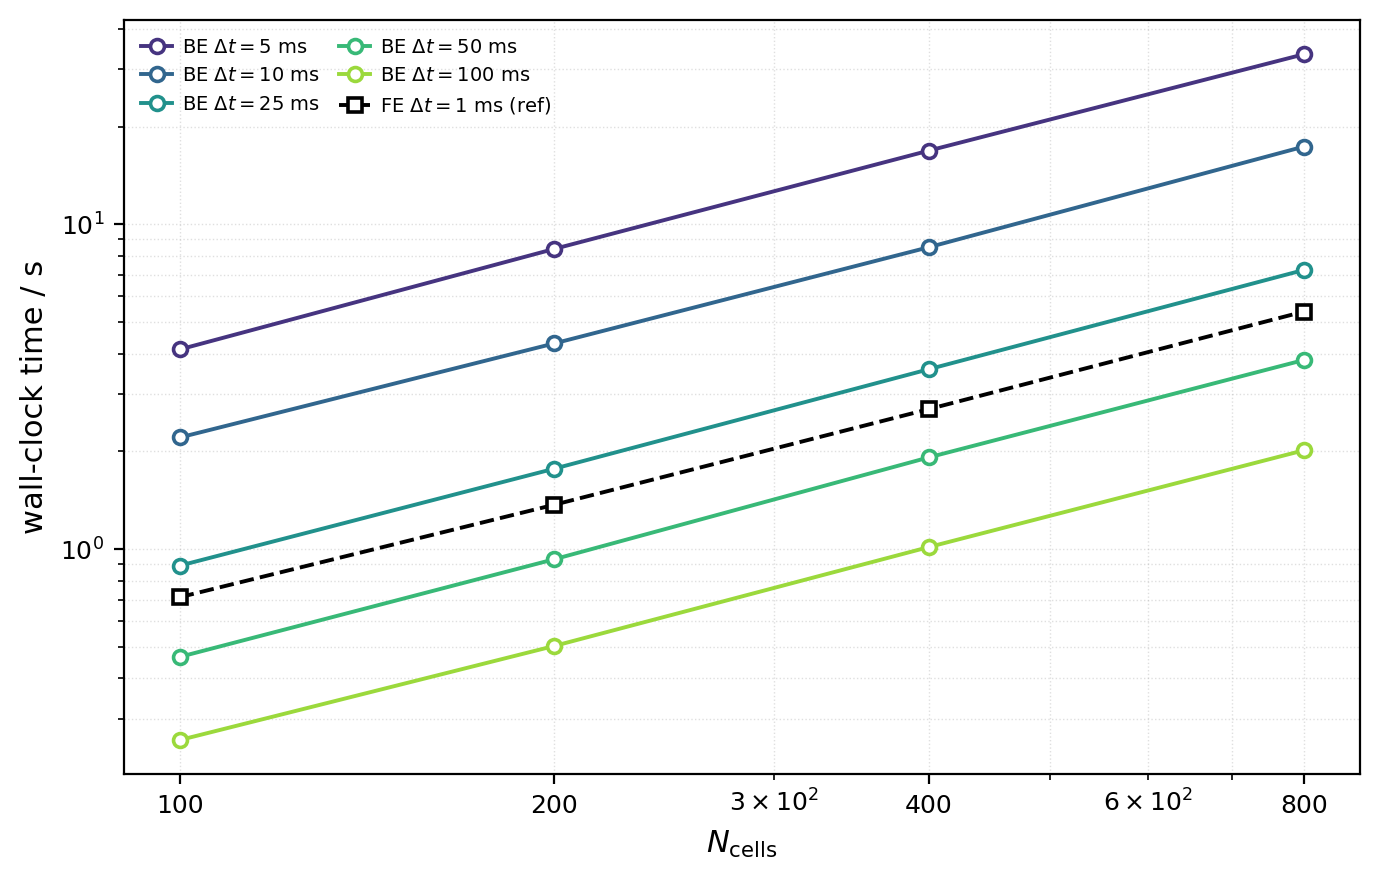
\includegraphics[width=0.95\textwidth]{figures/cpu_vs_n.png}
\caption{Wall-clock time vs grid resolution for forward Euler at \(\Delta t = \SI{1}{\milli\second}\) (dashed reference) and backward Euler at five time steps \(\Delta t \in \{5, 10, 25, 50, 100\}\,\si{\milli\second}\) (solid lines, viridis palette). All solvers integrate the real eight-reaction model from \(t = 0\) to \(t_\mathrm{end} = \SI{50}{\second}\).}\label{fig:cpu_vs_n}
\end{figure}

\Cref{fig:cpu_vs_n} shows the result. The structure of the comparison is itself unsurprising: all six curves --- the forward-Euler reference (dashed) and the five backward-Euler sweeps at increasing \(\Delta t\) (solid, viridis) --- follow the same slope-one scaling in log-log coordinates, because the per-step work of the banded Newton iteration scales linearly with \(\mathrm{NEQ} = N_\mathrm{cells}\cdot N_s\), and the total wall-clock time is therefore proportional to \(N_\mathrm{cells}\) at any fixed \(\Delta t\). The vertical spacing between the backward-Euler curves is set by the time-step ratio: doubling \(\Delta t\) approximately halves the wall time, since the typical Newton iteration count per step is essentially independent of \(\Delta t\) (\(\approx 25\) RHS evaluations per step at every grid in the sweep). What the comparison resolves is where backward Euler crosses the forward-Euler reference.

The forward-Euler reference falls between the backward-Euler curves at \(\Delta t = \SI{25}{\milli\second}\) and \(\Delta t = \SI{50}{\milli\second}\). At \(N_\mathrm{cells} = 400\), for instance, forward Euler at \(\Delta t = \SI{1}{\milli\second}\) takes \SI{2.7}{\second}, against \SI{3.6}{\second} for backward Euler at \(\Delta t = \SI{25}{\milli\second}\) and \SI{1.9}{\second} at \(\Delta t = \SI{50}{\milli\second}\). The crossover lies near \(\Delta t \approx \SI{25}{\milli\second}\) on this model and is independent of \(N_\mathrm{cells}\) across the tested range --- the two scaling laws are parallel, so the relative ordering of the integrators does not depend on grid resolution. The decisive moment of the test is at the largest backward-Euler step tested. At \(\Delta t = \SI{100}{\milli\second}\), backward Euler advances the real model to \(t_\mathrm{end} = \SI{50}{\second}\) in \SI{2.0}{\second} at \(N_\mathrm{cells} = 800\) against \SI{5.4}{\second} for forward Euler at the same grid --- a 2.7-fold acceleration that takes backward Euler from the slowest fixed-step integrator at its default settings (\cref{fig:test1_walltime}) to the fastest of the three at a tuned step.
% ===========================================================================
\section{Discussion and Solver Recommendation}\label{sec:ch4_discussion}
% ===========================================================================

The three numerical tests above converge on a single solver recommendation for the present model. \Cref{fig:test2_error} establishes that all three solvers reach the same spatial-discretisation floor at every grid: forward Euler, backward Euler, and DLSODE are accuracy-equivalent at any target \(N_\mathrm{cells}\) on the linear test problem. \Cref{fig:test1_walltime} then ranks them by cost on the real eight-reaction stiff model: forward Euler is the fastest of the three at every grid in the sweep, with backward Euler approximately a factor of three slower and DLSODE either marginally competitive at \(N_\mathrm{cells} = 100\) or, at higher resolutions, materially penalised by the BDF-order-collapse pathology described above. For a target relative error of \(\sim 10^{-3}\) (corresponding to \(N_\mathrm{cells} \approx 400\) in the error plot), forward Euler integrates the real model in \SI{2.6}{\second}, against \SI{8.2}{\second} for backward Euler and \SI{28.6}{\second} for DLSODE. The recommendation is therefore forward Euler at the default \(\Delta t = \SI{1}{\milli\second}\) --- the cheapest of the three integrators at the established accuracy floor. This recommendation comes with two important caveats.

\newpage

The first concerns the scope of the accuracy ranking, which is established on the linear simplified PFR and cannot be transposed verbatim to the stiff Arrhenius chemistry of the real model, where the time-integration error of forward Euler at \(\Delta t = \SI{1}{\milli\second}\) might no longer be below the spatial floor. A direct measurement of the time-integration error on the real model would require an analytical reference for the eight-reaction system, which does not exist; the indirect ranking provided by the second test is therefore the strongest accuracy claim available within the scope of this work. Within that limitation, the empirical result is unambiguous: at the engineering-relevant grids around \(N_\mathrm{cells} \approx 400\), forward Euler at the default \(\Delta t = \SI{1}{\milli\second}\) agrees with the DLSODE reference to within the spatial-discretisation floor of \cref{fig:test2_error}, and at materially lower wall-clock-time cost. 

The recommendation comes at a cost: the user must keep \(\Delta t\) within the conditional stability bound of forward Euler --- a discipline that adaptive methods like DLSODE assume on the user's behalf, and that backward Euler dispenses with through unconditional A-stability. \Cref{fig:cpu_vs_n} sharpens the picture further: when the user is willing to find a large stable time step for backward Euler --- here, \(\Delta t = \SI{100}{\milli\second}\) is stable and converges Newton at every grid tested --- backward Euler is the fastest of the three integrators on this model, displacing forward Euler from the top of the wall-clock ranking. The default-configuration ranking and the tuned ranking therefore disagree, and the choice between them is a deployment decision rather than a numerical one.

The second caveat looks forward rather than back. The recommendation rests on the present kinetic scheme and on the isothermal assumption --- eight Arrhenius reactions at a fixed operating temperature, which together leave the chemistry-induced stiffness within reach of forward Euler at \(\Delta t = \SI{1}{\milli\second}\). Two model extensions, both realistic next steps from the present work, would push the comparison the other way. The first is a more detailed reaction mechanism --- more species, a wider spread of activation energies, the chemistry one would adopt to model pyrolytic gas faithfully. The second is to relax the isothermal assumption and couple an energy balance to the species equations, so that the temperature, and through the Arrhenius dependence the rate constants, become part of the state vector --- a regime where local temperature excursions can amplify rate constants by orders of magnitude across a single integration step. Either extension would grow the stiffness of the right-hand side and tighten forward Euler's conditional-stability bound on \(\Delta t\).

\newpage

In the limit where the chemical timescale falls below the present transport-dominated bound, forward Euler will either choke or be forced into impractically small steps, and the constant per-step overhead of an implicit method becomes economical by comparison. DLSODE is built for exactly this regime: adaptive BDF order and predictor--corrector step-size control absorb the stiffness without user intervention, and the wall-clock-time penalty seen in \cref{fig:test1_walltime} on the present model would then be the price paid for robustness on a problem where the explicit scheme is no longer admissible. For either model extension the comparison would need to be re-run; based on what we see here, the ranking is likely to flip, with DLSODE moving ahead of forward Euler. On the present model, however, the answer is forward Euler.
